\section{Mathematical Background}


% ===== Slide 1 (Navier–Stokes) =====
\begin{secframe}
\small
\textcolor{red_unipd}{\Large General Form of Navier--Stokes Equations}

\vspace{0.6em}

\begin{alertblock}{Equations}
\[
\begin{cases}
\dfrac{\partial \rho}{\partial t}
+ \nabla\!\cdot\!(\rho \mathbf{u}) = 0,\\[16pt]

\dfrac{\partial (\rho \mathbf{u})}{\partial t}
+ \nabla\!\cdot\!(\rho \mathbf{u} \otimes \mathbf{u})
= -\nabla p + \nabla\!\cdot\!\boldsymbol{\Sigma} + \rho \mathbf{g},\\[16pt]

\dfrac{\partial E}{\partial t}
+ \nabla\!\cdot\!((E+p)\mathbf{u})
= \nabla\!\cdot\!(\boldsymbol{\tau}\!\cdot\!\mathbf{u})
- \nabla\!\cdot\!\mathbf{q} + \rho \mathbf{u}\!\cdot\!\mathbf{g}
\end{cases}
\]
\end{alertblock}

\end{secframe}




% ===== New Slide 3: Physical Meaning -- Mass Conservation =====
\begin{secframe}
\small
\textcolor{red_unipd}{\Large Conservation Laws: Mass}

\vspace{0.8em}

\begin{alertblock}{Continuity equation -- Mass Conservation}
\[
\dfrac{\partial \rho}{\partial t} + \nabla\!\cdot\!(\rho \mathbf{u}) = 0
\]
\end{alertblock}

\begin{block}{Term definitions}
\begin{itemize}
  \item \(\rho\): fluid density \([\text{kg·m}^{-3}]\)
  \item \(\mathbf{u} = (u,v,w)\): velocity field \([\text{m·s}^{-1}]\)
  \item \(\nabla\!\cdot\!(\rho \mathbf{u})\): divergence of mass flux
  \item \(\partial \rho / \partial t\): local time rate of change of density
\end{itemize}
\end{block}
\end{secframe}




% ===== Slide 4: Physical Meaning -- Momentum Conservation =====
\begin{secframe}
\small
\textcolor{red_unipd}{\Large Conservation Laws: Momentum}

\vspace{0.8em}

\begin{alertblock}{Newton’s second law -- Momentum equation}
\[
\dfrac{\partial (\rho \mathbf{u})}{\partial t}
+ \nabla\!\cdot\!(\rho \mathbf{u}\otimes\mathbf{u})
= -\nabla p + \nabla\!\cdot\!\boldsymbol{\Sigma} + \rho \mathbf{g}
\]
\end{alertblock}

\begin{block}{Term definitions}
\begin{itemize}
  \item \(\rho \mathbf{u}\): momentum density \([\text{kg·m}^{-2}\text{·s}^{-1}]\)
  \item \(\nabla\!\cdot\!(\rho \mathbf{u}\otimes\mathbf{u})\): convective momentum transport
  \item \(-\nabla p\): pressure gradient force per unit volume
  \item \(\boldsymbol{\Sigma}\): viscous stress tensor \([\text{Pa}]\)
  \item \(\rho \mathbf{g}\): body force density (e.g. gravity) \([\text{N·m}^{-3}]\)
\end{itemize}
\end{block}
\end{secframe}




% ===== Slide 5: Physical Meaning -- Energy Conservation =====
\begin{secframe}
\small
\textcolor{red_unipd}{\Large Conservation Laws: Energy}

\vspace{0.8em}

\begin{alertblock}{Energy equation (first law of thermodynamics)}
\[
\dfrac{\partial E}{\partial t}
+ \nabla\!\cdot\!((E+p)\mathbf{u})
= \nabla\!\cdot\!(\boldsymbol{\tau}\!\cdot\!\mathbf{u})
- \nabla\!\cdot\!\mathbf{q}
+ \rho \mathbf{u}\!\cdot\!\mathbf{g}
\]
\end{alertblock}

\begin{block}{Term definitions}
\begin{itemize}
  \item \(E = \rho\!\left(e + \tfrac{1}{2}|\mathbf{u}|^2\right)\): total energy density (internal + kinetic)
  \item \(p\): pressure \([\text{Pa}]\)
  \item \(\boldsymbol{\tau}\): stress tensor (viscous + pressure)
  \item \(\mathbf{q}\): heat flux vector \([\text{W·m}^{-2}]\)
  \item \(\rho \mathbf{u}\!\cdot\!\mathbf{g}\): work done by body forces
\end{itemize}
\end{block}
\end{secframe}




% ===== Slide 6 =====
\begin{secframe}
\small
\textcolor{red_unipd}{\Large Newtonian Hypotheses and Constitutive Relations}

\begin{alertblock}{Viscous Stress}
\[
\begin{cases}
\boldsymbol{\Sigma} = \mu\left(\nabla \mathbf{u} + (\nabla \mathbf{u})^T\right) + \lambda (\nabla\!\cdot\!\mathbf{u}) \mathbf{I},\\[4pt]
\boldsymbol{\tau} = \boldsymbol{\Sigma} - p \mathbf{I}
\end{cases}
\]
\end{alertblock}

\begin{alertblock}{Heat Flux}
\[
\mathbf{q} = -k \nabla T
\]
\end{alertblock}

\begin{alertblock}{Internal Energy}
\[
E = \rho\left(e + \dfrac{1}{2}|\mathbf{u}|^2\right)
\]
\end{alertblock}

\end{secframe}




% ===== Slide 7 (Navier–Stokes with Constitutive Relations Expanded) =====
\begin{secframe}
\small
\textcolor{red_unipd}{\Large General Form with Constitutive Relations Expanded}

\vspace{0.6em}

\begin{alertblock}{Equations (Newtonian, compressible, viscous fluid)}
\[
\begin{cases}
\dfrac{\partial \rho}{\partial t}
+ \nabla\!\cdot\!(\rho \mathbf{u}) = 0,\\[16pt]

\rho\!\left(
\dfrac{\partial \mathbf{u}}{\partial t}
+ (\mathbf{u}\!\cdot\!\nabla)\mathbf{u}
\right)
= -\nabla p
+ \nabla\!\cdot\!\Big[
\mu\!\left(\nabla \mathbf{u} + (\nabla \mathbf{u})^T\right)
+ \lambda (\nabla\!\cdot\!\mathbf{u})\mathbf{I}
\Big]
+ \rho \mathbf{g},\\[20pt]

\dfrac{\partial }{\partial t}\!
\left[\rho\!\left(e + \dfrac{1}{2}|\mathbf{u}|^2\right)\right]
+ \nabla\!\cdot\!
\left[\rho\!\left(e + \dfrac{1}{2}|\mathbf{u}|^2\right)\mathbf{u} + p\mathbf{u}\right]
= \\ \nabla\!\cdot\!
\Big\{
\mu\!\left(\nabla \mathbf{u} + (\nabla \mathbf{u})^T\right)\!\cdot\!\mathbf{u}
+ \lambda (\nabla\!\cdot\!\mathbf{u})\mathbf{u}
- k\nabla T
\Big\}
+ \rho \mathbf{u}\!\cdot\!\mathbf{g}
\end{cases}
\]
\end{alertblock}

\end{secframe}




% ===== Slide 8 =====
\begin{secframe}
\small
\textcolor{red_unipd}{\Large Why Navier--Stokes Matters in Neural PDEs}

\vspace{0.6em}

\begin{block}{Central role in neural modeling}
The Navier--Stokes system unifies diffusion (viscous term),  
advection (nonlinear term), and incompressibility (constraint).  
Each paper tests neural architectures by simplifying or approximating parts of this system:
\begin{itemize}
  \item \textbf{PINNs:} direct enforcement of differential operators;
  \item \textbf{FNOs:} operator learning across time steps of Navier–Stokes;
  \item \textbf{NFTM:} learned iterative refinement mimicking PDE rollouts.
\end{itemize}
\vspace{0.4em}
Through these methods, the goal is to determine whether deep neural architectures can reproduce  
\textit{the stability and accuracy of physical solvers} for complex spatio-temporal dynamics.
\end{block}
\end{secframe}






% ===== Slide 1 =====
\begin{secframe}
\small
\textcolor{red_unipd}{\Large Burgers Equation as a Simplified Model}

\vspace{0.6em}

\begin{alertblock}{Equation}
\[
\begin{cases}
  u_t + u u_x + v u_y = \nu (u_{xx} + u_{yy}), \\
  v_t + u v_x + v v_y = \nu (v_{xx} + v_{yy})
\end{cases}
\]
\end{alertblock}

\vfill

\begin{block}{Hypotheses}
\(\nabla p=\mathbf{0}\). \quad
1D reduction: \(\mathbf{u}=(u(x,t),0)\). \quad
Self-advection: \(u\,\partial_x u\).
\end{block}

\vspace{0.5em}

\begin{block}{Einstein notation}
$u_t = \frac{\partial u}{\partial t}$, $u_x = \frac{\partial u}{\partial x}$, $u_{xx} = \frac{\partial^2 u}{\partial x^2}$, etc.
\end{block}

\end{secframe}

% ===== Advection Frame =====
\begin{secframe}
\small
\textcolor{red_unipd}{\Large Advection}

\vspace{0.6em}

\begin{block}{Advection Terms}
\begin{itemize}
    \item \textbf{$u u_x$, $v v_y$, $u v_x$, $v u_y$}: Nonlinear advection terms.
    \item Represent transport of velocity due to the flow itself.
\end{itemize}
\end{block}

\begin{figure}[h]
    \centering
    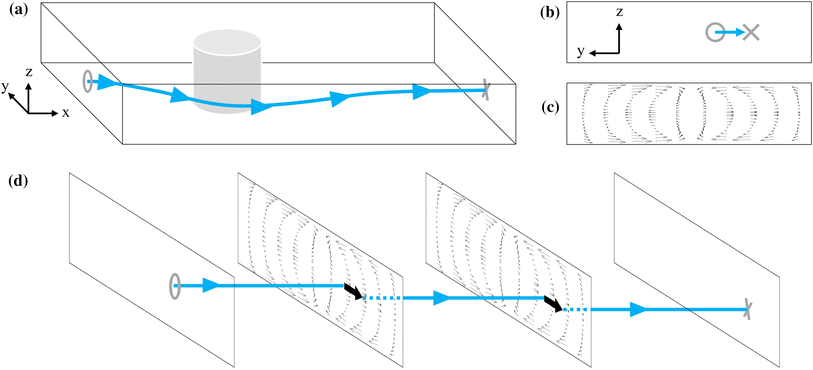
\includegraphics[width=0.7\linewidth]{images/theory/advection.png}
\end{figure}

\end{frame}

% ===== Diffusion Frame =====
\begin{frame}{2D Burgers Equation}
\small
\textcolor{red_unipd}{\Large Diffusion}

\vspace{0.6em}

\begin{block}{Diffusion Terms}
\begin{itemize}
    \item \textbf{$\nu (u_{xx} + u_{yy})$, $\nu (v_{xx} + v_{yy})$}: Diffusion terms.
    \item Model the spreading and smoothing of velocity due to viscosity $\nu$.
\end{itemize}
\end{block}

\begin{figure}[h]
    \centering
    
\includegraphics[width=0.7\linewidth]{images/theory/diffusion.png}
\end{figure}


\end{secframe}

% ===== Balance Frame =====
\begin{secframe}
\small
\textcolor{red_unipd}{\Large Pressure gradient}

\vspace{0.6em}

\begin{alertblock}{Pressure Gradient Terms}
  The huge Hypotheses here is \(\nabla p=\mathbf{0}\), so there is no effect of the pressure in the equation. \\
  \( \Rightarrow \) Only the initial velocity has an influence on the evolution of the system
\end{alertblock}

\begin{example}
  Consider a scenario where the initial velocity is constant across the domain on airfoil shape. \\
  Since \(\nabla p=\mathbf{0}\), the pressure gradient does not influence the flow. \\
  The flow will not change over time, remaining constant as per the initial condition.
\end{example}



\end{secframe}

% ===== Slide 2 =====
\begin{secframe}
\small
\textcolor{red_unipd}{\Large Numerical Simulation}

\vspace{0.6em}

\begin{block}{Description}
\begin{itemize}
  \item Implements the PDE directly using finite difference methods.
  \item Discretizes space and time; updates velocity fields step by step.
  \item Parameters: grid size, time step, viscosity, initial/boundary conditions.
\end{itemize}
\end{block}

\begin{alertblock}{Finite Difference Schemes}
\begin{itemize}
  \item Forward difference (time): $u_t \approx \frac{u_{i,j}^{n+1} - u_{i,j}^n}{\Delta t}$
  \item Central difference (space): $u_x \approx \frac{u_{i+1,j}^n - u_{i-1,j}^n}{2\Delta x}$
  \item Central difference (second derivative): $u_{xx} \approx \frac{u_{i+1,j}^n - 2u_{i,j}^n + u_{i-1,j}^n}{\Delta x^2}$
\end{itemize}
\end{alertblock}

\end{secframe}




\section{2D Neural Model}

% ===== Slide 1: Overview =====
\begin{secframe}
\small
\textcolor{red_unipd}{\Large 2D Neural Network Pipeline}

\vspace{0.6em}

\begin{block}{Goal}
Learn to predict 2D Burgers trajectories $\mathbf{u}(x,y,t)$ from short histories.
\end{block}

\begin{block}{Pipeline}
\begin{itemize}
  \item Load generated 2D dataset (train/test) with viscosity labels $\nu$.
  \item Train a Transformer-based controller on sequences of frames.
  \item Evaluate: trajectory rollout and error over time.
\end{itemize}
\end{block}

\end{secframe}



% % ===== Slide 2: Dataset =====
% \begin{secframe}
% \small
% \textcolor{red_unipd}{\Large 2D Dataset Configuration}

% \vspace{0.6em}

% \begin{block}{Source}
% Generated 2D Burgers dataset with separate train/test folders.
% \end{block}

% \begin{block}{Key settings}
% \begin{itemize}
%   \item Dataset type: generated 2D samples.
%   \item History length: $3$ frames.
%   \item Batch size: $4$.
%   \item Input grid inferred from data: $(C, H, W)$.
% \end{itemize}
% \end{block}

% \end{secframe}



% % ===== Slide 3: Model =====
% \begin{secframe}
% \small
% \textcolor{red_unipd}{\Large 2D Transformer Controller}

% \vspace{0.6em}

% \begin{block}{Architecture}
% TransformerController2D with patch-based tokens.
% \end{block}

% \begin{block}{Hyperparameters}
% \begin{itemize}
%   \item Patch radius: $r=0$ \;\; ($\text{patch size} = C(2r+1)^2$).
%   \item Hidden size: $64$.
%   \item Output channels: $C$.
%   \item Chunk size: $5$ (sequential rollout).
% \end{itemize}
% \end{block}

% \end{secframe}



% % ===== Slide 4: Training =====
% \begin{secframe}
% \small
% \textcolor{red_unipd}{\Large Training Setup}

% \vspace{0.6em}

% \begin{block}{Training loop}
% \begin{itemize}
%   \item $40$ epochs of supervised learning.
%   \item Loss tracked over epochs and visualized after training.
%   \item Optional model loading/saving for checkpoints.
% \end{itemize}
% \end{block}

% \begin{alertblock}{Objective}
% Minimize trajectory prediction error over time for the chosen $\nu$.
% \end{alertblock}

% \end{secframe}



% % ===== Slide 5: Evaluation =====
% \begin{secframe}
% \small
% \textcolor{red_unipd}{\Large Evaluation and Visualization}

% \vspace{0.6em}

% \begin{block}{Evaluation}
% \begin{itemize}
%   \item Select a target viscosity $\nu$ (fixed or random).
%   \item Rollout prediction vs. ground truth on test data.
%   \item Compute relative $\ell_2$ error over time.
% \end{itemize}
% \end{block}

% \begin{block}{Outputs}
% \begin{itemize}
%   \item Animated 2D fields (true, predicted, error).
%   \item Error curve summarizing stability across time.
% \end{itemize}
% \end{block}

% \end{secframe}